\documentclass{article}
\usepackage[utf8]{inputenc}

\title{Identifying ATLAS stream members with a Bayesian mixture model}
\author{Andrew Li | 1006675625 | andrewp.li@mail.utoronto.ca}
\date{May 15, 2023}

\usepackage{amsfonts}
\usepackage{amsmath}
\usepackage{url}
\usepackage{graphicx}
\usepackage{float}
\usepackage{listings}

\usepackage{geometry}
 \geometry{
 left=25mm,
 right=25mm,
 top=25mm,
 bottom=25mm,
 }

\usepackage{physics}
\usepackage{verbatim}
\usepackage{wrapfig}
\usepackage{hyperref}
\usepackage{natbib}

\usepackage{minted}
\usepackage{xcolor}
\definecolor{LightGray}{gray}{0.9}

\bibliographystyle{aasjournal}

\begin{document}

\maketitle

\vspace{-2em}

\section{Introduction}

This report aims to determine stellar members of the ATLAS-Aliqa Uma stream, henceforth referred to as ATLAS. Data from the Southern Stellar Stream Spectroscopic Survey ($S^5$) \citep{10.1093/mnras/stz2731}, and Gaia DR2 \citep{refId0} is used to construct a Bayesian mixture model, from which we can determine the membership probabilities of each individual star. We will also compare our results to the identified parameters and members in \citep{2021ApJ...911..149L}.\\

First, we select our data and perform cuts to ensure good quality measurements. We then convert the celestial equatorial $(\alpha, \delta)$ to spatial stellar stream coordinates $(\phi_1,\phi_2)$ defined by \citep{Shipp_2019}. This conversion is given by
\begin{align}
    \begin{pmatrix}
        \cos(\phi_1)\cos(\phi_2)\\\sin(\phi_1)\cos(\phi_2)\\\sin(\phi2)
    \end{pmatrix}=
    \begin{pmatrix}
        0.83697865& 0.29481904& -0.4610298\\
        0.51616778& -0.70514011& 0.4861566\\
        0.18176238& 0.64487142& 0.74236331
    \end{pmatrix}\times
    \begin{pmatrix}
        \cos(\alpha)\cos(\delta)\\\sin(\alpha)\cos(\delta)\\\sin(\delta)
    \end{pmatrix}.\label{eq:1}
\end{align}
The velocity measurements, given as heliocentric $(v_\text{hel})$ are also converted to be with respect to the Galactic Standard of Rest $(v_\text{GSR})$, which will be completed using a function described in \citet{Price-Whelan_2023}.\\

We now construct a mixture model, consisting of one stream component and one background component. The model is based on three measurement quantities: $v_\text{GSR}$, the proper motion in right ascension $(\mu_\alpha)$, and the proper motion in declination $(\mu_\delta)$. Each quantity has a mean and scattering, which will be modelled into a Gaussian. Additionally, the means of these quantities will be a quadratic function of $\phi_1$ for the stream component. We use a Markov Chain Monte Carlo (MCMC) sampler to optimize these parameters. Once they are determined, we can find the membership probabilities of each star.\\

This report is structured as follows. In Section 2, we present the data from $S^5$, Gaia DR2, and \citet{2021ApJ...911..149L}, along with the quality cuts made. In Section 3, we present the mixture model and perform MCMC to find the best-fit parameters. The membership probabilities are subsequently determined. In Section 4, we discuss our results and compare to \citet{2021ApJ...911..149L}, and conclude in Section 5. The methods used in this report will be completed through Python using Jupyter Notebook. The Python libraries used are \texttt{numpy} \citep{harris2020array}, \texttt{matplotlib} \citep{Hunter:2007}, \texttt{astropy} \citep{2022ApJ...935..167A}, \texttt{emcee} \citep{Foreman_Mackey_2013}, \texttt{corner} \citep{dan_foreman_mackey_2023_7808805}, \texttt{scipy} \citep{2020SciPy-NMeth}, and \texttt{schwimmbad}. 

\section{Data}

The data used in this report is collected from $S^5$ and Gaia DR2. This data is provided as a FITS file and the stars in spatial proximity to the ATLAS stream can be extracted by the key \texttt{`object\_name'==`ATLAS'}. $v_\text{GSR}$ is also determined using the function described in \citet{Price-Whelan_2023}, and the stream coordinates using Equation \ref{eq:1}.\\

Quality cuts are also performed to exclude both poor measurements and stars far away from the known parameters. We select stars with \texttt{`good\_star'==1}, $[\text{Fe/H}]<-1.5$, $|v_\text{GSR}|<250 \text{ km s}^{-1}$, $|\mu_\alpha\cos\delta|<4\text{ mas yr}^{-1}$, and $|\mu_\delta|<4\text{ mas yr}^{-1}$. After these cuts, we are left with 1044 stars.\\

Data of known members of ATLAS is also collected from \citet{2021ApJ...911..149L}. This data is provided as a FITS file and these stars are selected by the key \texttt{`regionname'==`AAU'}. The $v_\text{GSR}$, $\phi_1$, $\phi_2$ transformations are also applied similarly. All of this data can be seen in Figure \ref{fig:1}.

\begin{figure}[H]
\begin{center}
    \includegraphics[width=\textwidth]{figures/fig 1.png}
\end{center}
    \vspace{-2em}
    \caption{The data members used in this report. For all panels, grey markers represent $S^5$ members that did not pass the quality cuts described in Section 2, and black markers represent those that did. The red markers indicate the members of ATLAS identified by \citet{2021ApJ...911..149L}. All panels all share an axis of the stellar stream coordinate $\phi_1$, in units of degrees. The panels (top to bottom) show $\phi_2$ in degrees, $v_\text{GSR}$ in km s$^{-1}$, $\mu_\alpha\cos\delta$ in mas yr$^{-1}$, and $\mu_\delta$ in mas yr$^{-1}$.}
    \label{fig:1}
\end{figure}

\section{Data analysis}

\subsection{Modelling}

The mixture model used will consist of two components, which we will call `stream' and `background'. The first parameter $p_\text{stream}$, will be the fraction of stars in the stream component. For the stream component, three measurement qualities will be used: $v_\text{GSR}$, $\mu_\alpha\cos\delta$, and $\mu_\delta$. Each of these will be represented by two parameters, mean and variance, which compose a Gaussian distribution. Additionally, the means for each of these quantities will be a quadratic function of $\phi_1$. For example, $v_\text{GSR}$, the mean will be represented as
\begin{align}
    v_\text{GSR}=v_\text{GSR,1}+v_\text{GSR,2}x+v_\text{GSR,3}x^2,
\end{align}
where $x=\phi_1/10^\circ$ and $\phi_1$ is in units of degrees and $v_\text{GSR}$ is in km s$^{-1}$. The quadratic coefficients for the proper motion components are defined similarly. This gives the stream component 12 parameters. For the background component, we will also use a Gaussian for each quantity, but this time there will be no dependence on $\phi_1$ for the means. This gives another 6 parameters, for a total of 19 parameters. These parameters can be seen in Table \ref{table:1}.\\

We will now construct the probability function to be used by the MCMC sampler. The probability function is the product of the prior and the likelihood. The prior will simply be hard cutoffs for each parameter, determined by inspection of Figure 1 and results from \citet{2021ApJ...911..149L}. The selected bounds are also shown in Table \ref{table:1}. The likelihood functions for the stream and background components are products of each of the three Gaussians for each measurement as stated above. They are then scaled by their respective contributions $(p_\text{stream},1-p_\text{stream})$ and multiplied together.\\

Our initial guesses for the parameters are formulated both visually and using values from \citet{2021ApJ...911..149L}. Using \texttt{minimize} from \texttt{scipy.optimize}, we minimize the negative probability function to get a better estimate for our parameters. Finally, we maximize the likelihood function using \texttt{EnsembleSampler} from \texttt{emcee}, run with 64 walkers and 2000 iterations. The initial guesses, \texttt{scipy} results and \texttt{emcee} results are all shown in Table \ref{table:1}. The corner plot of the MCMC sampling result is also shown in Figure \ref{fig:2}.\\

\vspace{-0.5em}
\begin{table}[h]
\begin{center}
\caption{Summary of the modelling and analysis completed in Section 3. In the leftmost column, the 19 parameters are shown, along with their representation in the code and their units. The subscript $b$ indicates the parameter is part of the background component. The priors set for these parameters are shown next, followed by their initial guesses. The results of both \texttt{scipy.optimize.minimize} and \texttt{emcee} are shown in the last two columns.}
\label{table:1}
\vspace{1em}
\begin{tabular}{ |c|c|c|c|c| } 
\hline
Parameter (var in code) [units] & Prior & Initial guess &\texttt{scipy} results & \texttt{emcee} results\\
\hline
$p_\text{stream}$ (\texttt{pstream}) [unitless] & $[0,1]$ & 0.20 & 0.08 & $0.10\pm0.01$\\
$v_\text{GSR,1}$ (\texttt{v1}) [km s$^{-1}$]& $[-160,100]$ & $-120$ & $-132$ & $-131\pm1$\\
$v_\text{GSR,2}$ (\texttt{v2}) [km s$^{-1}$]& $[-1,4]$ & 0.07 & $-0.05$ & $2.29\pm0.57$\\
$v_\text{GSR,3}$ (\texttt{v3}) [km s$^{-1}$]& $[0,10]$ & 5.68 & 2.88 & $2.30\pm0.60$\\
$\log_{10}[\sigma_{v_\text{GSR}}]$ (\texttt{lsigv}) [km s$^{-1}$]& $[-1,4]$ & 1.40 & 0.72 & $0.67\pm0.04$\\
$(\mu_\alpha\cos\delta)_1$ (\texttt{pmra1}) [mas yr$^{-1}$]& $[-1,1]$ & $-0.10$ & $-0.19$ & $-0.17\pm0.02$\\
$(\mu_\alpha\cos\delta)_2$  (\texttt{pmra2}) [mas yr$^{-1}$]& $[-1,1]$ & 0.24 & $-0.31$ & $-0.32\pm0.02$\\
$(\mu_\alpha\cos\delta)_3$  (\texttt{pmra3}) [mas yr$^{-1}$]& $[-1,1]$ & 0.09 & $-0.08$ & $-0.08\pm0.02$\\
$\log_{10}[\sigma_{\mu_\alpha\cos\delta}]$ (\texttt{lsigpmra}) [mas yr$^{-1}$]& $[-1,3]$ & $-0.20$ & $-0.86$ & $-0.84\pm0.04$\\
$\mu_{\delta,1}$ (\texttt{pmdec1}) [mas yr$^{-1}$]& $[-2,0]$ & $-0.96$ & $-0.99$ & $-0.98\pm0.02$\\
$\mu_{\delta,2}$ (\texttt{pmdec2}) [mas yr$^{-1}$]& $[-1,1]$ & 0.07 & $-1.22$ & $-0.07\pm0.01$\\
$\mu_{\delta,3}$ (\texttt{pmdec3}) [mas yr$^{-1}$]& $[-1,1]$ & 0.07 & $0.05$ & $0.01\pm0.01$\\
$\log_{10}[\sigma_{\mu_{\delta}}]$ (\texttt{lsigpmdec}) [mas yr$^{-1}$]& $[-2,3]$ & $-0.50$ & $-0.85$ & $-0.98\pm0.04$\\
$v_\text{GSR,b}$ (\texttt{bv}) [km s$^{-1}$]& $[-50,50]$ & 20.0 & $10.9$ & $-3.03\pm3.25$\\
$\log_{10}[\sigma_{v_\text{GSR,b}}]$ (\texttt{lsigbv}) [km s$^{-1}$]& $[-1,4]$ & 2.00 & $1.99$ & $2.00\pm0.01$\\
$(\mu_\alpha\cos\delta)_b$ (\texttt{bpmra}) [mas yr$^{-1}$]& $[0,2]$ & 1.40 & 1.10 & $1.06\pm0.05$\\
$\log_{10}[\sigma_{(\mu_\alpha\cos\delta)}]$ (\texttt{lsigbpmra}) [mas yr$^{-1}$]& $[-1,3]$ & 0.20 & $0.18$ & $0.17\pm0.01$\\
$\mu_{\delta,b}$ (\texttt{bpmdec}) [mas yr$^{-1}$]& $[-4,0]$ & $-2.50$ & $-2.08$ & $-2.09\pm0.04$\\
$\log_{10}[\sigma_{\mu_{\delta,b}}]$ (\texttt{lsigbpmdec}) [mas yr$^{-1}$]& $[-2,3]$ & 0.00 & $0.01$ & $0.04\pm0.01$\\
\hline
\end{tabular}
\end{center}
\end{table}

\pagebreak

\begin{figure}[H]
\begin{center}
    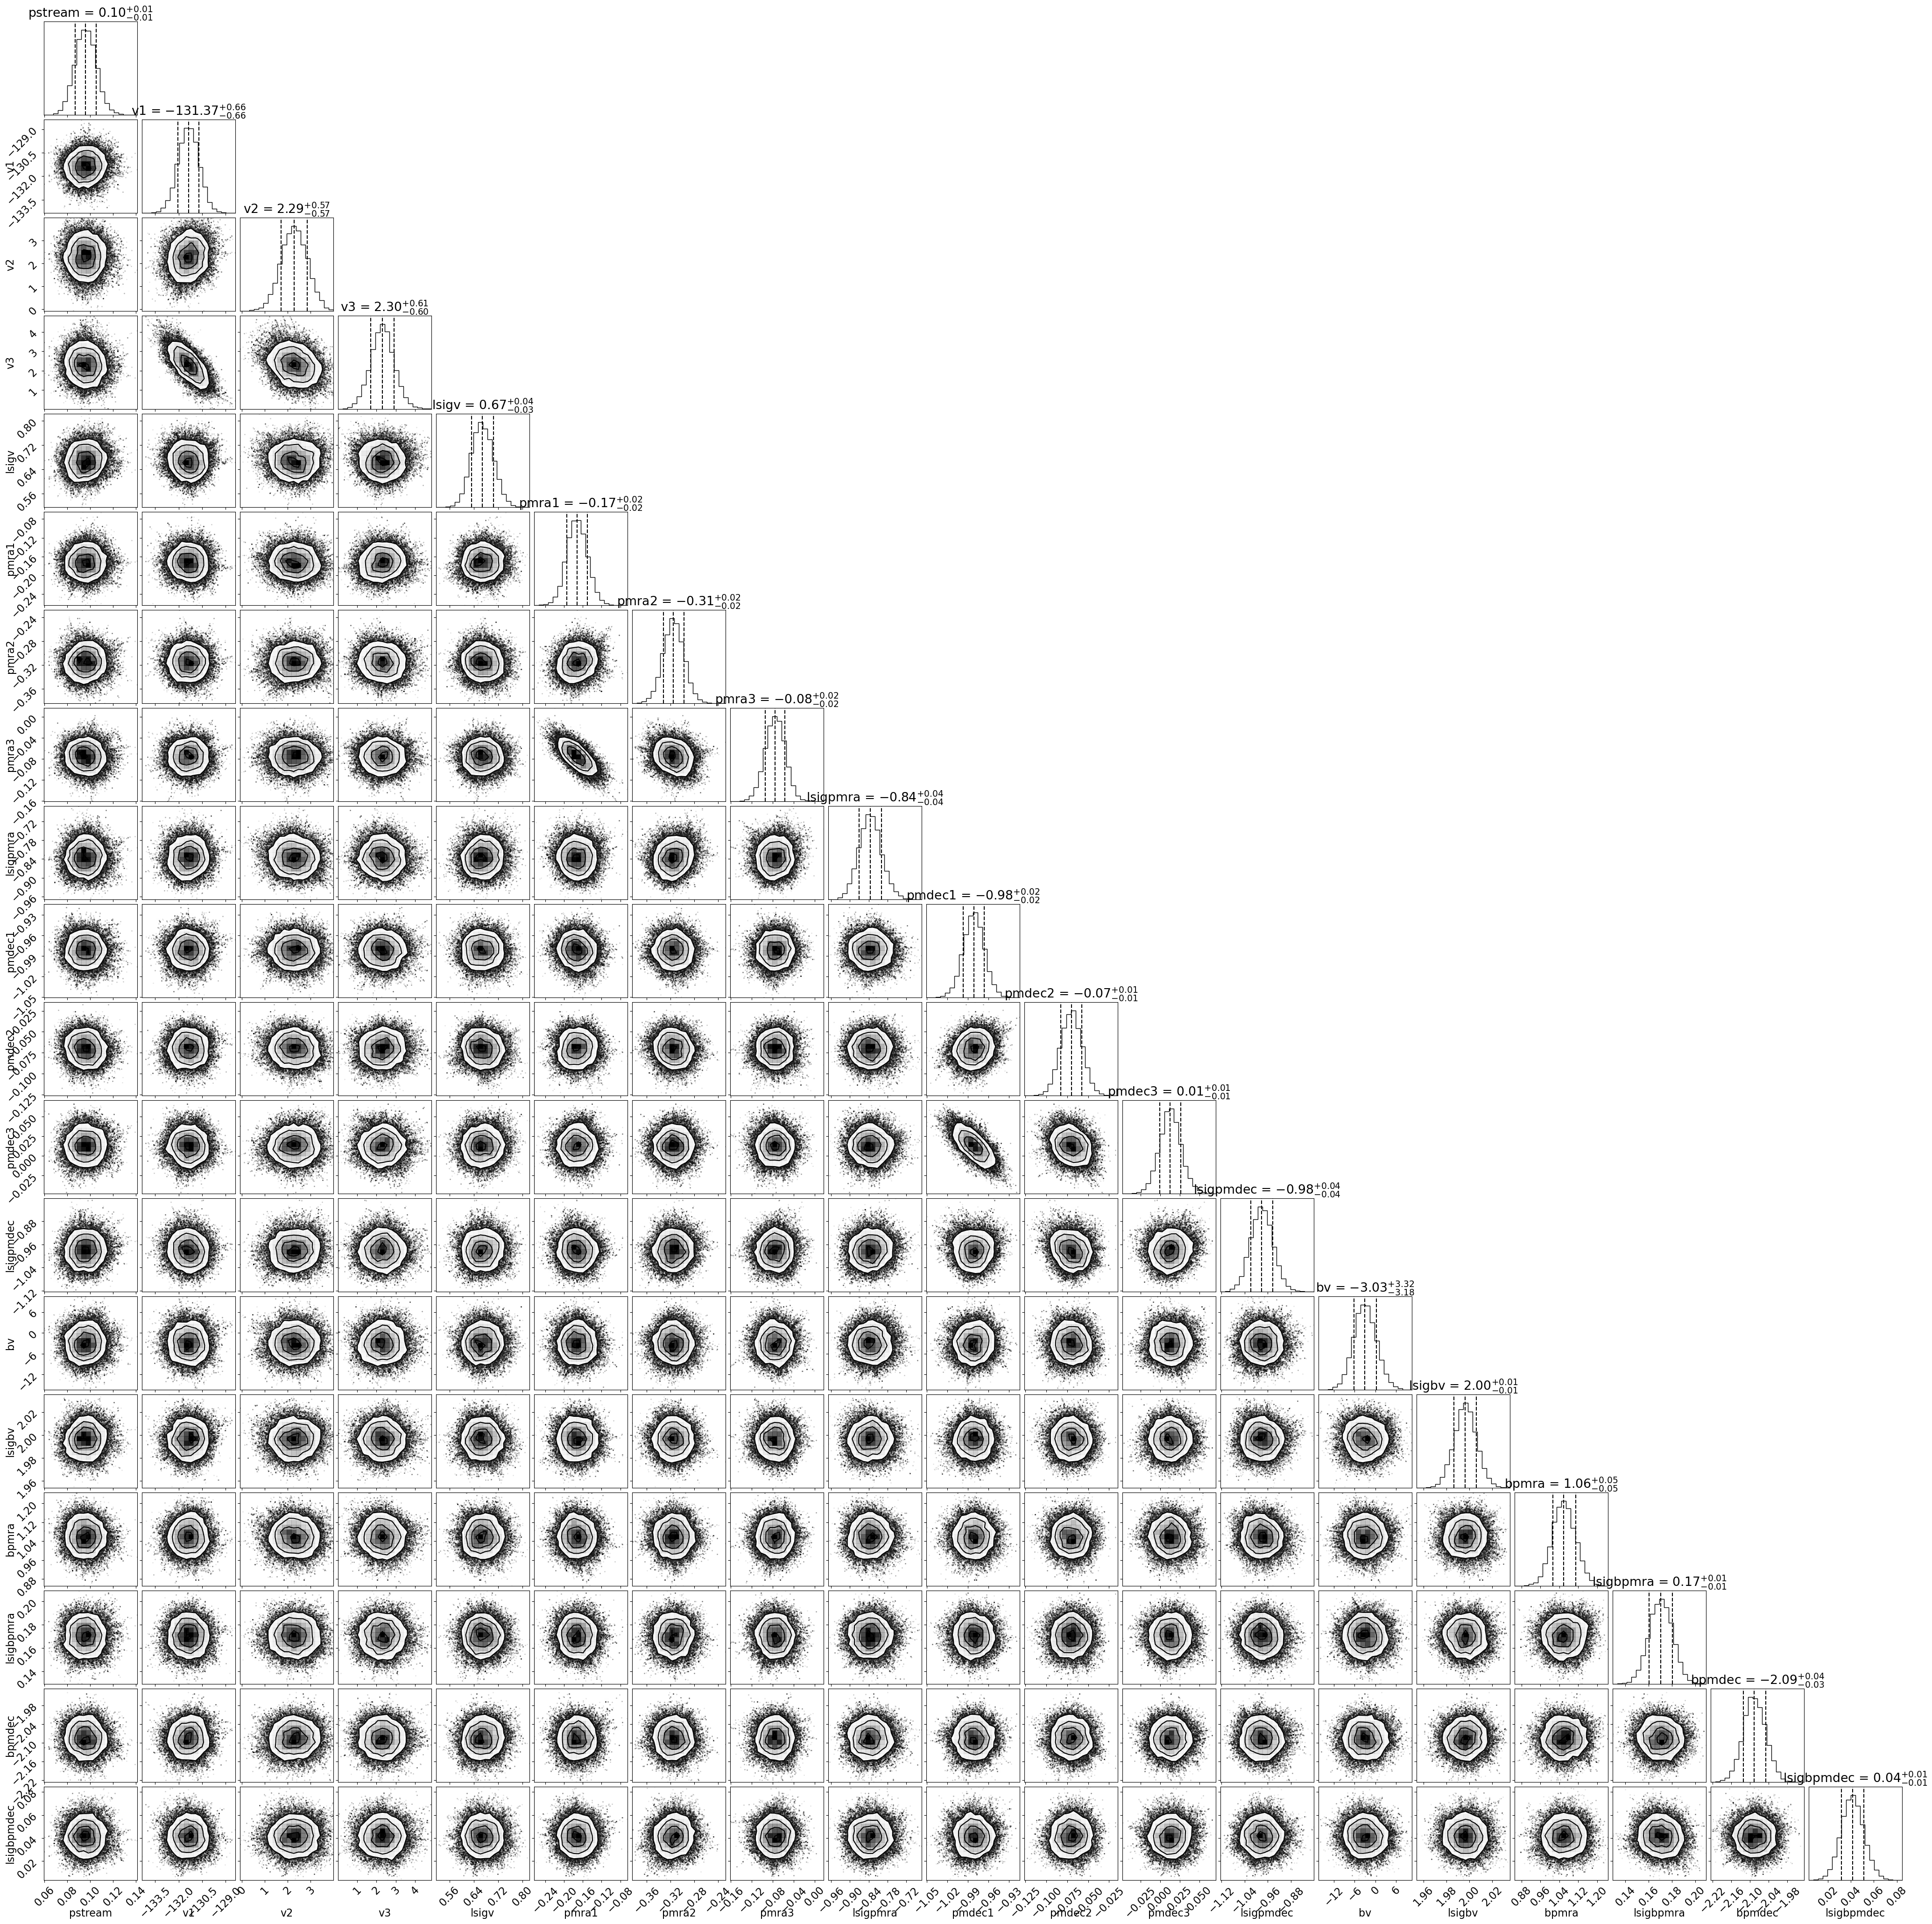
\includegraphics[width=\textwidth]{figures/fig 2.png}
\end{center}
    \vspace{-2em}
    \caption{The corner plot of the results of the MCMC sampler. The probability function and procedure used is described in Section 3.}
    \label{fig:2}
\end{figure}

\pagebreak

\subsection{Membership probability}

To find the membership probability, we can use the likelihood functions of the components $\mathcal{L}_\text{stream},\mathcal{L}_\text{background}$ as defined in Section 3.1. The membership probability $p$ is given by
\begin{align}
    p=\frac{p_\text{stream}\cdot\mathcal{L}_\text{stream}}{p_\text{stream}\cdot\mathcal{L}_\text{stream}+(1-p_\text{stream})\cdot\mathcal{L}_\text{background}}.
\end{align}
The membership probabilities of each star can be seen in Figure \ref{fig:3}.
\begin{figure}[H]
\begin{center}
    \includegraphics[width=\textwidth]{figures/fig 3.png}
\end{center}
    \vspace{-2em}
    \caption{The membership probabilities of stars in the $S^5$ data set, displaying all $p>0.1$ in accordance with the colorbar on the right. Displayed in grey are all stars where $p\leq0.1$. The axes are identical to those in Figure 1.}
    \label{fig:3}
\end{figure}

\pagebreak

\section{Discussion}

Overall the processes in this report ran smoothly. 92 stars were identified with $p>0.7$, which can be seen in Figure \ref{fig:4}. It can also be seen in this figure that there is considerable overlap between the identified stars and those determined in \citet{2021ApJ...911..149L}, which adds support to our findings. One potential issue can be seen in Figure \ref{fig:3}, where there is a noticeable lack of members with $0.1<p<0.8$. The reasons for this are unclear and are worth mentioning.\\

\begin{figure}[H]
\begin{center}
    \includegraphics[width=\textwidth]{figures/fig 4.png}
\end{center}
    \vspace{-2em}
    \caption{Members of stars in the $S^5$ data set ($p>0.7$) compared to the identified members in \citet{2021ApJ...911..149L}, displayed as red circles and blue triangles respectively.}
    \label{fig:4}
\end{figure}

Some areas for improvement can be considered. Firstly, our data cuts eliminated around 87\% of the sample population. The data cuts seem reasonable, as there is unlikely to be stream members at such high velocities or proper motions, but additional data could have been discarded nonetheless. Secondly, it is possible that a Gaussian fit for the background components may not be ideal. This can be seen in Figure \ref{fig:1}, which shows distributions for proper motion that seem more complicated. Similarly, the quadratic functions for the means of the stream component may find more success and accordance with \citet{2021ApJ...911..149L} if models with more degrees of freedom were considered. Lastly, the covariance between $\mu_\alpha\cos\delta$ and $\mu_\delta$ is not considered, although the effect of this on our results should not be large.

\section{Conclusion}

This report was able to determine 92 members of the ATLAS stream using a Bayesian mixture model. Stars close to the ATLAS stream were selected from $S^5$ and quality cuts were made. The stream coordinates of each star was determined, and the heliocentric velocities were converted with respect to the Galactic Standard of Rest. A 19 parameter mixture model was constructed and sampled using MCMC methods to find the best fit parameters. This model was used to determine the membership probability of each star, and those with $p>0.7$ were selected. Our results were in accordance with \citet{2021ApJ...911..149L}. Overall, this report was completed with relative success.

\bibliography{bibby}

\end{document}